\zexternaldocument{inleiding}
\zexternaldocument{analyse}
\zexternaldocument{evaluatie}

\chapter{IMP}
\label{sec:IMP}
Dit deel geeft een introductie in configuratiemanagementtools en IMP specifiek.
Configuratietools laten toe op een effici\"ente manier complexe IT-infrastructuren te onderhouden.
Sectie \ref{sec:configuratiemanagement} geeft een inleiding tot configuratiemanagement.
Sectie \ref{sec:IMP_werking} geeft meer uitleg over hoe IMP werkt en op welke vlakken dit verschilt met de werking van de huidige tools.

\section{Configuratiemanagement}
\label{sec:configuratiemanagement}
%CMS nog eens uitleggen, plaatsing van IMP binnen de andere tools?

\section{Werking}
\label{sec:IMP_werking}
Deze sectie beschrijft hoe een IMP-opstelling er uitziet en hoe een model opgesteld en uitgerold wordt.
Sectie \ref{sec:IMP_structuur} beschrijft de verschillende onderdelen van een gedistribueerd systeem dat gebruikt maakt van IMP, en hoe deze interageren.
Sectie \ref{sec:IMP_opstellen_model} geeft uitleg over het declaratief model dat de gebruiker opstelt.
Er wordt uitleg gegeven over de structuur van zo'n model, welke elementen er in voorkomen en hoe die elementen gevormd worden.
Daarna volgt uitleg over de verwerking van dat model tijdens het uitrolproces.

\subsection{Operationele structuur}
\label{sec:IMP_structuur}
Structureel bestaat IMP uit \'e\'en management server en verschillende agents.
De management server houdt het configuratiemodel bij.
Als de gebruiker het model wil exporteren zal de management server eerst dat model compileren en dan naar de verschillende agents versturen.

\subsection{Opstellen van het model}
\label{sec:IMP_opstellen_model}
Het configuratiemodel van IMP kan beschreven worden in twee delen: het configuratiemodel zelf en de bibliotheken.
In het configuratiemodel staat de infrastructuur die de gebruiker wenst te bekomen.
Deze bestaat uit een oplijsting van machines en de resources die moeten aanwezig zijn op die machines.
Deze resources kunnen in complexiteit vari\"eren van een simpele file tot een volledige webserver.

De verschillende types resources worden gedefini\"eerd als entiteiten in bibliotheken. 
Zo is er de standaardbibliotheek ``std'' met onder andere de definitie van een host, een bestand, een service,\ldots
Het is belangrijk een duidelijk onderscheid te maken tussen entiteiten en implementaties uit bibliotheken en resources gedefini\"eerd in een configuratiemodel.
Entiteiten defini\"eren de naam en attributen van een domeinconcept.
De implementatie van een entiteit specifi\"eert uit welke andere entiteiten ze is opgebouwd.

De resources vermeld in het model zijn instanties van de entiteiten uit de bibliotheken.
Een entiteit kan \'e\'en of meerdere reeds bestaande entiteiten overerven.
Zo kan de gebruiker makkelijk verschillende entiteiten combineren, zonder limiet op het aantal niveaus van overerving.
Een visuele voorstelling van de overerving en de resources binnen een entiteit en zijn implementatie is te vinden op figuur \ref{fig:model_hierarchie}.
Hier is duidelijk te zien dat er sprake is van twee hi\"erarchie\"en: de gedefini\"eerde entiteiten kunnen van elkaar overerven en vormen zo een opwaartste hi\"erarchie.
Een implementatie is een lijst van ge\"instantieerde enteteiten (resources dus) die elk weer kunnen bestaan uit verzamelingen van resources.
Dit vormt een neerwaartse hi\"erarchie.

\begin{figure}[h]
    \begin{center}
    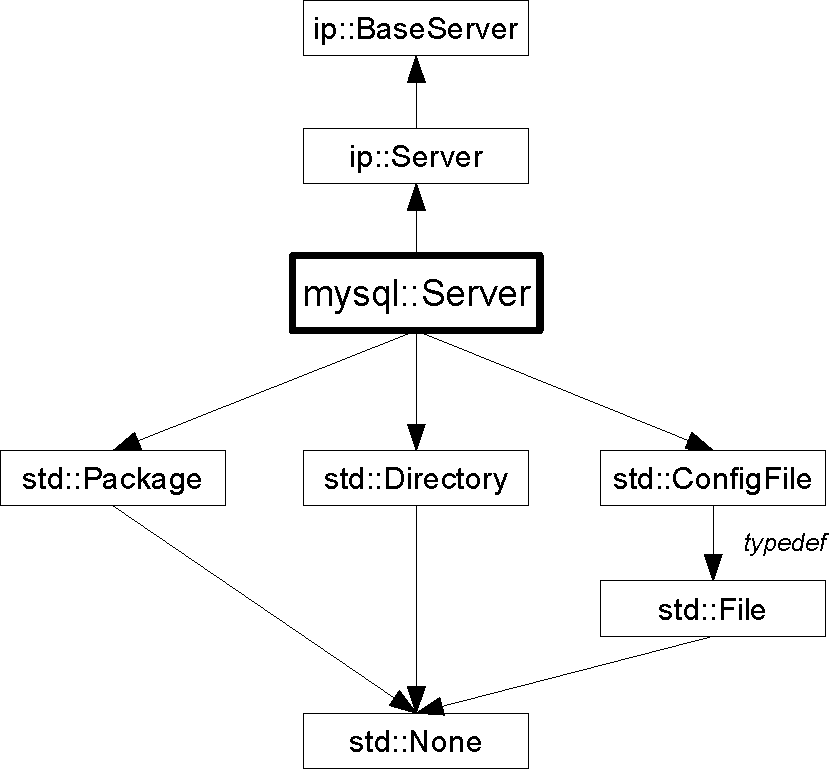
\includegraphics[width=0.6\textwidth]{images/model_hierarchie.pdf}
    \caption{Voorstelling van de hi\"erarchie die aanwezig is tussen de verschillende entiteiten.
            De mysql-server erft over van de Server -en BaseServerentiteit uit de ip-bibliotheek.
            De resources gedefini\"eerd binnen de implementatie van een mysqlserver erven ook over van andere entiteiten.}
    \label{fig:model_hierarchie}
    \end{center}
\end{figure}

Een voorbeeld van een eenvoudige bibliotheek is deze van de MySQL-database:

\lstinputlisting[label=listing:mysql_model]{listings/mysql_model}

Net zoals de meeste bibliotheken begint deze met een oplijsting van de verschillende entiteiten die gedefini\"eerd worden.
Zoals daarnet gezegd kunnen entiteiten opgebouwd worden aan de hand van andere entiteiten. 
Hier wordt een MysqlServer entiteit gedefini\"eerd als een uitbreiding op de Server entiteit uit de ip bibliotheek.
Entiteiten kunnen attributen hebben, in dit geval heeft een Database een naam, een gebruiker en een wachtwoord.
Daarbovenop komen nog de attributen die gedefini\"eerd zijn voor een Server.

Regel 13 toont een belangrijke feature van IMP: relaties.
Relaties zijn een vorm van domeinspecifieke informatie over hoe twee entiteiten in relatie staan met elkaar. 
In dit geval weet de gebruiker dat voor elke MySQL-server nul of meerdere databases moeten gespecifi\"eerd worden, en dat voor elke database exact \'e\'en MySQL-server moet gespecifi\"eerd worden.
Aan de hand van deze informatie kan IMP onder andere bij het compileren nakijken of aan deze relatie voldaan is en zoniet dit melden aan de gebruiker.
Dit reduceert de kans op configuratiefouten. 
Concreet zal in het configuratiemodel naast de gewone attributen van een mysqlserver of een database nog een extra attribuut moeten opgegeven worden: respectievelijk de database of server waarmee ze in relatie staat.
Andere CMS laat niet toe dit soort informatie op te geven en kunnen dit soort checks dus niet doen.
Deze relaties zullen in sectie \ref{sec:relaties} ook gebruikt worden om het uitrolproces te optimaliseren.

Het laatste deel van een bibliotheek bestaan uit de implementaties van de ervoor gedefini\"eerde entiteiten.
In deze implementaties worden de entiteiten opgebouwd aan de hand van instanties van andere entiteiten.
In dit geval bestaat een MysqlServer-entiteit uit een instantie van het mysql-server pakket, de mysqld-service en een paar configuratiebestanden-en mappen.
Deze komen allemaal uit de std-bibliotheek.
In de declaratie van deze resources is ook te zien hoe de attributen hun waarden krijgen. 
Op regel 30 staat de declaratie van de mysqld-service.
De attributen ``name'', ``state'' en ``onboot'' worden in de bibliotheek zelf opgegeven.
Het attribuut ``host'' wordt opgegeven door de gebruiker bij het invullen van de attributen van een MysqlServer in het configuratiemodel.

Een voorbeeld van een configuratiemodel staat in listing \ref{listing:drupal_main}.
Dit model stelt een installatie van Drupal voor op \'e\'en host.
Voor Drupal zijn een werkende web -en databaseserver nodig.

\lstinputlisting[label=listing:drupal_main]{listings/drupal_main}

Regel 1 toont dat dit model een host bevat met een bepaalde hostname (``server'') en een bepaald IP-adres.
Alle elementen van de drupal installatie zullen geplaatst worden op deze host.

De volgende 2 regels specificeren dat op de daarnet gedefini\"eerde host vm1 een httpd-server en een mysql-database moeten aanwezig zijn.
Zoals daarnet besproken moet enkel nog het ``host''-attribuut van een mysql-server ingevuld worden door de gebruiker, de andere attributen werden in de bibliotheek al ingevuld.
De declaratie van de drupalsite zelf (regel 15) toont ook duidelijk dat relaties ook attributen introduceren: zowel ``vhost'' als ``database'' zijn attributen die door een relatie gespecificeerd worden.
\todo{belang van opgeven van alle informatie, hier of bij de heuristieken?}

\subsection{Uitrollen van het model}
\label{sec:IMP_uitrollen}
Als het model volledig opgesteld is kan de gebruiker het uitrollen.
Dit proces bestaat uit meerdere stappen.
Eerst komt een kort overzicht van het proces, waarna dieper wordt ingegaan op elke stap.

Zoals gezegd bestaat het uitrolproces uit meerdere stappen:
\begin{enumerate}
    \item Compilatie van het model
        \begin{enumerate}
            \item IMP vereenvoudigt de resources stap per stap tot de basis (bestanden, mappen, pakketten en services)
            \item De verschillende dependency managers worden opgeroepen en doen verdere aanpassingen aan het model
        \end{enumerate}
    \item verdeling van het model
    \item Toepassen van configuratieaanpassingen
        \begin{enumerate}
            \item De resources die geen vereisten hebben worden uitgerold \todo{vereisten/relaties vermelden}
            \item De uitgerolde resources worden verwijderd uit de vereisten van andere resources
            \item Stap 1 en 2 worden herhaald tot alle resources uitgerold zijn.
        \end{enumerate}
\end{enumerate}

\paragraph{Compilatie van het model}
In de compilatiestap zal IMP de samengestelde resources stapsgewijs omzetten tot basisresources zoals bestanden, pakketten en services.
Zoals in sectie \ref{sec:IMP_opstellen_model} vermeld laat IMP namelijk toe om entiteiten te combineren om zo herbruikbare concepten te defini\"eren. (Zie ook figuur \ref{fig:model_hierarchie}.)
In de compilatiestap wordt dus de omgekeerde weg terug gevolgd.
Dit proces wordt ``concept refinement'' genoemd en wordt grafisch voorgesteld op figuur \ref{fig:concept_refinement}.

\begin{figure}[h]
    \begin{center}
    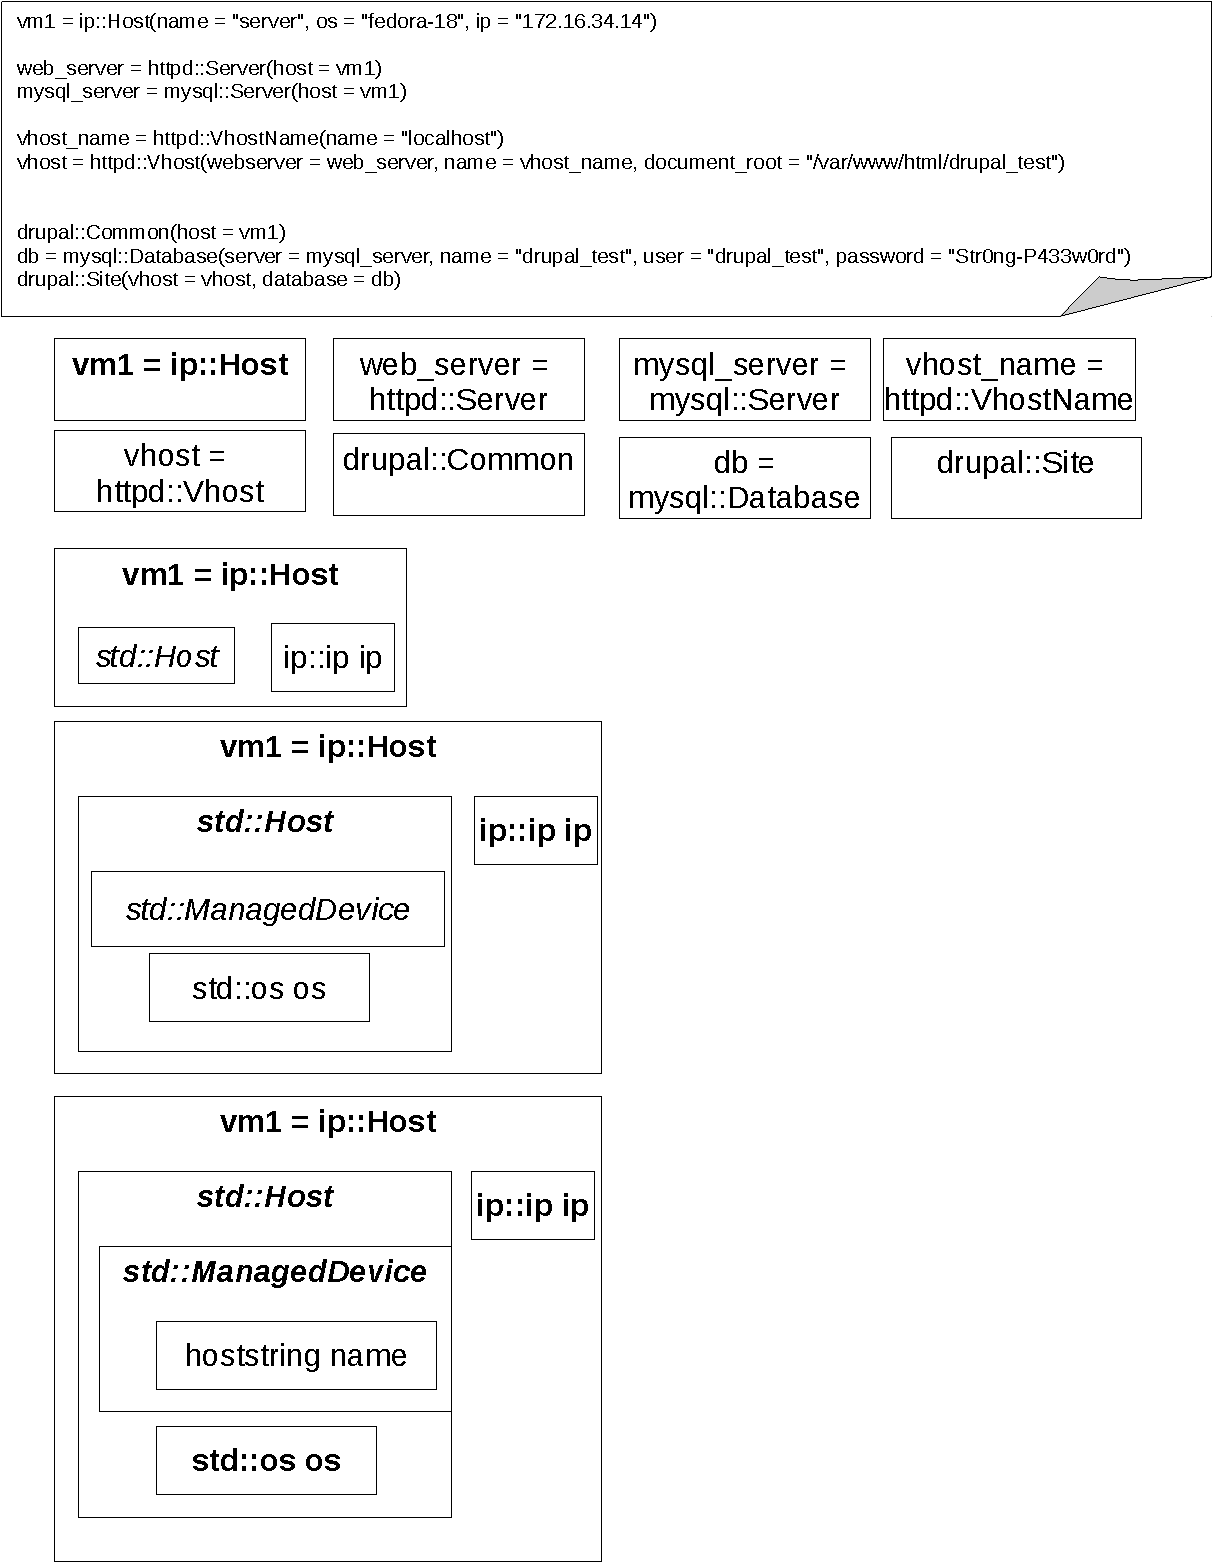
\includegraphics[width=0.6\textwidth]{images/concept_refinement.pdf}
    \caption{Voorstelling van hoe de hoger-niveau resources worden gerefined tot lager-niveau resources en hun attributen.}
    \label{fig:concept_refinement}
    \end{center}
\end{figure}

Als het laagste niveau bereikt is en enkel nog basisresources overblijven is de eerste stap van het compilatieprocess af.
Nu krijgen de dependency managers de kans om nog aanpassingen te doen aan het model.
Dependency managers zijn Python functies die de gebruiker kan schrijven als deel van een bibliotheek.
Deze krijgen als argumenten het hoogste niveau van het model, het configuratiemodel, en de lijst met uiteindelijke resources, het resourcemodel.\todo{termen vroeger vermelden}
Daarmee kan de gebruiker extra aanpassingen uitvoeren op de modellen voordat het verder uitgerold wordt.
In deze thesis worden de dependency managers gebruikt om de gevonden heuristieken toe te passen.

\paragraph{verdeling van het model}
Eens het model opgesteld is moet elke host zijn deel van het model met de relevante resources ontvangen.
De communicatie tussen de management server en de verschillende agents die actief zijn op de hosts gebeurt via een AMQP-bus (zie figuur \ref{fig:IMP_architectuur}).
De agents schrijven zich in voor alle resources die gedefini\"eerd zijn voor hun host en ontvangen zo enkel het voor hen relevante deel van het model.
Als een agent een resource uitgerold heeft zet hij ook een bericht op de AMQP-bus zodat andere agents weten als een vereiste voldaan is.
In tegenstelling tot andere CMS is er dus communicatie tussen de verschillende agents, wat toelaat op een gedistribueerde manier de vereisten correct af te handelen. \todo{Vergelijking maken met andere CMS? Hier of in related work?}

\begin{figure}[h]
    \begin{center}
    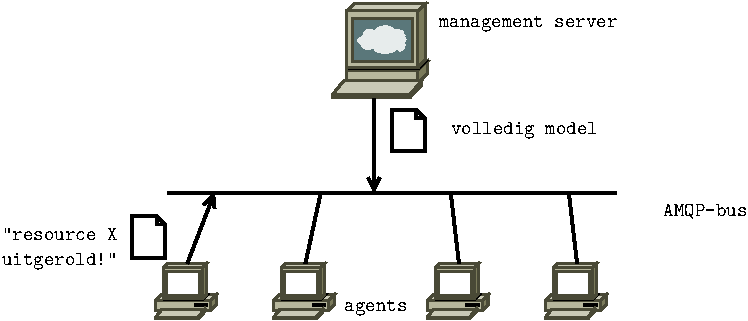
\includegraphics[width=0.6\textwidth]{images/IMP_architectuur.pdf}
    \caption{Deployment model van IMP met de management server en de agents, allemaal verbonden via een AMQP-bus}
    \label{fig:IMP_architectuur}
    \end{center}
\end{figure}

\paragraph{convergentie}
\todo{Schrijven}

%twee soorten model, configmodel en resourcemodel

  %Welke resources heb je
  %Verschillende niveaus in het model
    %Desired state config model
    %Deployment model
    %Per machine model
    % -> concept refinement
  %Dependency managers
    %wat
    %waar/wanneer
